\documentclass{article}
\usepackage{fancyhdr}
\usepackage{lipsum}  
\usepackage{listings} 
\usepackage{xcolor}   
\usepackage{amsmath}
\usepackage{enumitem}
\usepackage{graphicx}
\usepackage{caption}
\usepackage{verbatim}

% Define macros for title and author
\newcommand{\thetitle}{STAT 641 \\ Homework 4}
\newcommand{\theauthor}{Keegan Smith}

\title{\thetitle}
\author{\theauthor}

\pagestyle{fancy}
\fancyhf{}  % Clear all header and footer fields
\fancyhead[L]{\nouppercase{\rightmark}}
\fancyhead[C]{\thetitle}  % Title in the center
\fancyhead[R]{\theauthor}  % Your name on the right

\lstset{ %
  backgroundcolor=\color{lightgray},   % choose the background color
  basicstyle=\ttfamily\small,          % size of fonts used for the code
  keywordstyle=\color{blue},           % color for keywords
  commentstyle=\color{green},          % color for comments
  stringstyle=\color{red},             % color for strings
  numbers=left,                        % where to put the line-numbers
  numberstyle=\tiny\color{gray},       % style for line-numbers
  stepnumber=1,                        % the step between two line-numbers
  numbersep=5pt,                       % how far the line-numbers are from the code
  frame=single,                        % adds a frame around the code
  rulecolor=\color{black},             % frame color
  breaklines=true,                     % automatic line breaking
  breakatwhitespace=false,             % automatic breaks should only happen at whitespace
  showspaces=false,                    % don't show spaces in the code
  showstringspaces=false,              % don't show spaces in strings
  showtabs=false,                      % don't show tabs in the code
}

\begin{document}

\maketitle
\section*{Problem 1}
First of all, in the data, none of the entries are marked with status == 0, so I will be treating this data as uncensored. \\
\begin{enumerate}
\item 
\begin{enumerate}[label=\alph*)]
\item the trimmed mean is 886.7853403141361 and the untrimmed mean is 955.3713080168776. This would suggest that the data has some extreme values to the right, and is right skewed. \\
\item the survival function is: \\
\[
S(t) = 1 - F(t)
\]
We can derive $F(t)$ from the pdf, (and since $t$ is a time any probability for $t < 0$ is 0, so we are only considering $t \geq 0$): \\
\begin{align*}
F(t) &= \int_{0}^{t}\lambda e^{-\lambda x} \\
&= (-e^{-\lambda x})_{0}^{t} \\
&= (-e^{-\lambda t} - (-1)) \\
&= 1 - e^{-\lambda t}
\end{align*}
So we have: \\
\begin{align*}
S(t) &= e^{-\lambda t} \\
\ln(S(t)) &= -\lambda t \\ 
\end{align*}
So if $S(t)$ is a good estimate, then the plot $t$ vs $\ln(S(t))$ should be a linear plot with slope: \\
\[
\frac{t}{-\lambda t} = \frac{1}{-\lambda}
\]
The actual plot is: \\
\begin{figure}[htbp]
    \centering
    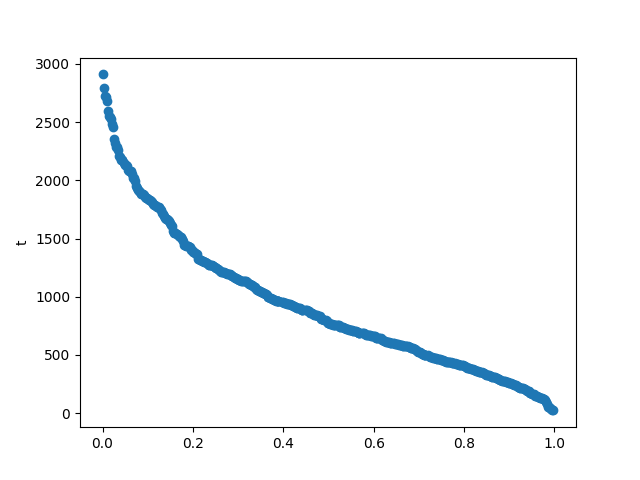
\includegraphics[width=0.8\textwidth]{fig_1.png}
\end{figure}
\item We have the likelihood function: \\
\begin{align*}
L(\lambda;y) &= \Pi_{k = 0}^{n-1}\lambda e^{-\lambda y_k} \\
&= \lambda^ne^{\sum_{k=0}^{n-1}-\lambda y_k} \\
&= \lambda^ne^{-\lambda \cdot \sum_{k=0}^{n-1} y_k} \\
\end{align*}
The log likelihood function is then: \\
\begin{align*}
\ln(L(\lambda;y)) &= \ln(\lambda^ne^{-\lambda \cdot \sum_{k=0}^{n-1} y_k}) \\
&= \ln(\lambda^n) + (-\lambda \cdot \sum_{k=0}^{n-1} y_k) \\
&= n \cdot \ln(\lambda) -\lambda \cdot \sum_{k=0}^{n-1} y_k
\end{align*}
The derivative of the log likelihood function w.r.t $\lambda$ is: \\
\begin{align*}
\frac{d}{d\lambda} (n \cdot \ln(\lambda) -\lambda \cdot \sum_{k=0}^{n-1} y_k) &= n \cdot \frac{1}{\lambda} - \sum_{k=0}^{n-1} y_k \\
&= \frac{n}{\lambda} - \sum_{k=0}^{n-1} y_k
\end{align*}
Solving for the maximum: \\
\begin{align*}
\frac{n}{\lambda} - \sum_{k=0}^{n-1} y_k &= 0 \\
\lambda &= \frac{n}{\sum_{k=0}^{n-1} y_k} \\
&= \frac{1}{\mu}
\end{align*}
Thus the MLE estimate for $\lambda$ is $\frac{1}{955.3713} \approx 0.001047$
\item The exponential distribution estimated probability that a male will have a survival time $>$ 1200 is: \\
\begin{align*}
P(t > 1200) &= 1 - P(t \leq 1200) \\
&= 1 - F(t) \\
&= 1 - (1 - e^{-\lambda t}) \\
&= e^{-0.001047 \cdot 1200}\\ 
&= 0.2846770212809416
\end{align*}
The distribution free estimate is: \\
\begin{align*}
P(t > 1200) &= 1 - P(t \leq 1200) \\
&= 1 - F(1200) \\
&= 1 - 0.7257383966244726 \\
&= 0.2742616033755274
\end{align*}
\item First I'm just going to derive the Quantile function to make this slightly less painful: \\
\begin{align*}
z &= 1 - e^{-\lambda t} \\
-z + 1 = e^{-\lambda t} \\
\ln(-z + 1) &= -\lambda t \\
t &= \frac{\ln(-z + 1)}{-\lambda}
\end{align*}
So: \\
\[
Q(z) = \frac{\ln(-z + 1)}{-\lambda} \\
\]
Thus we have the MLE median: \\
\begin{align*}
Q(.5) &= \frac{\ln(-.5 + 1)}{-0.001047} \\
&= 662.0316910792219
\end{align*}
MLE IQR: \\
\begin{align*}
Q(.75) - Q(.25) &= \frac{\ln(-.75 + 1)}{-0.001047} - \frac{\ln(-.25 + 1)}{-0.001047} \\
&= 1049.2954046495795
\end{align*}
Distribution free median is 833, the IQR is 793. These vary greatly from the MLE estimates for the exponential distribution, implying that the exponential distribution may not be a great fit for the distribution of survival times. \\
\end{enumerate}
\item The distribution free estimates for the mean and standard deviation are simply the sample mean and standard deviation respectively, which are: $955.371308$ and $634.253830$ for males, and $896.506977$ and $569.495299$ for females. \\
\item For males the estimated median is 833 and the MAD is 567.8280207561156. For females the estimated median is 759 and the MAD is 558.9325426241661.\\
\begin{verbatim}
def mad(data):
  data = np.asarray(data)
  c = np.median(data)
  deviations = np.abs(data - c)
  raw_mad = np.median(deviations)
  return raw_mad / 0.6745
\end{verbatim}
\item The above results would imply that the female average survival time is less than the male average survival time and that the variability in survival times is less for females than for males.
\end{enumerate}
\section*{Problem 2}
\begin{enumerate}
\item This experiment is using random censoring since there isn't a specified time when the experiment was stopped, patients could leave at random times. Knowing this, we will use Kaplan-Meier to approximate the survival function. Using the R code from handout 7, we get the following survival functions for treatments 1 and 2: \\
\begin{figure}[htbp]
    \centering
    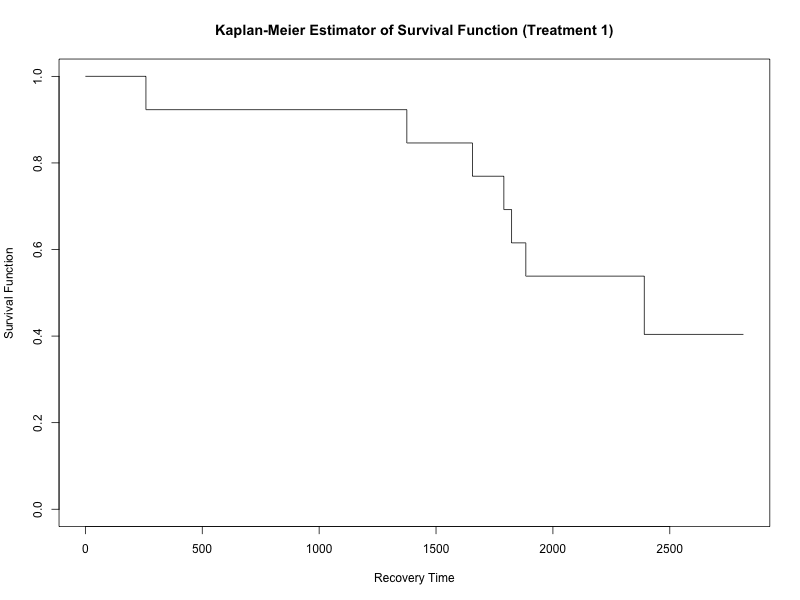
\includegraphics[width=0.8\textwidth]{treatment1_survival.png}
\end{figure}
\begin{figure}[htbp]
  \centering
  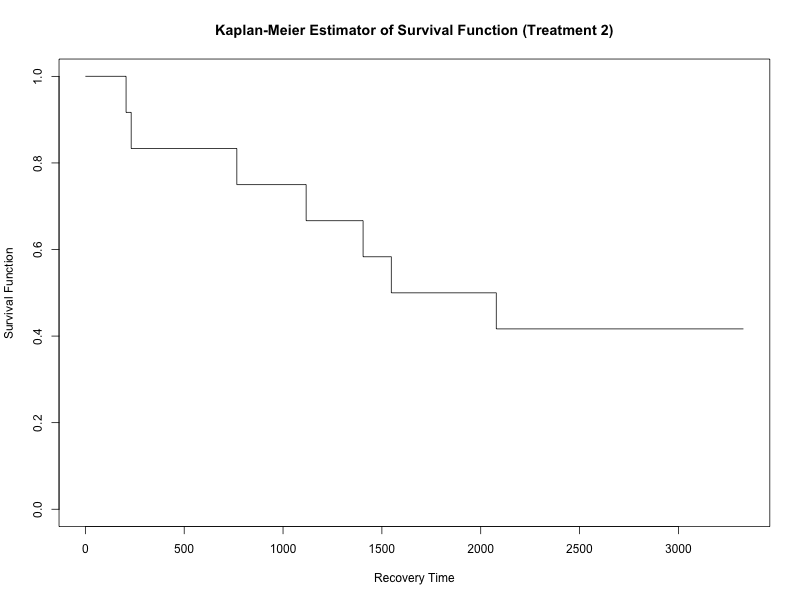
\includegraphics[width=0.8\textwidth]{treatment2_survival.png}
\end{figure}
\newpage
\item The estimated mean from the survival function for treatment 1 is 2135 and the estimated median is 2391. The estimated mean from the survival function for treatment 2 is 2000 and the estimated median is 1814. \\
\item From the estimated mean recovery times, it would appear that treatment 2 is more effective than treatment 1. \\
\item The estimated mean and median for treatment 1 are 1596.857142857143 and 1375 respectively, for treatment 2 they are 1050.4285714285713 and 1117 respectively. \\
\end{enumerate}
The code used for this problem is below: \\
\begin{verbatim}
library(survival)

df <- data.frame(
  time   = c(2391, 2815, 1884, 1656, 2184, 2118, 1905, 1375, 259, 1790, 2413, 2761, 1823),
  status = c(1, 0, 1, 1, 0, 0, 0, 1, 1, 1, 0, 0, 1)
)

km.fit <- survfit(Surv(time, status) ~ 1, data = df)

print(km.fit)
png("treatment1_survival.png", width=800, height=600)

plot(km.fit,conf.int=FALSE,log=FALSE,
main="Kaplan-Meier Estimator of Survival Function (Treatment 1)",xlab="Recovery Time",
ylab="Survival Function")
summary(km.fit)
print(km.fit, print.rmean=TRUE, rmean="individual")

df <- data.frame(
  time   = c(2312, 2501, 2691, 1548, 3329, 2154, 766, 1405, 1117, 232, 206, 2079),
  status = c(0, 0, 0, 1, 0, 0, 1, 1, 1, 1, 1, 1)
)

km.fit <- survfit(Surv(time, status) ~ 1, data = df)

print(km.fit)
png("treatment2_survival.png", width=800, height=600)

plot(km.fit,conf.int=FALSE,log=FALSE,
main="Kaplan-Meier Estimator of Survival Function (Treatment 2)",xlab="Recovery Time",
ylab="Survival Function")
summary(km.fit)
print(km.fit, print.rmean=TRUE, rmean="individual")
\end{verbatim}
\section*{Problem 3}
\begin{enumerate}
\item A (type 1 censoring)\\
\item B (type 2 censoring)\\
\item C (right censoring) \\
\item C (random censoring) \\
\item A (left censoring since you know the patient got the disease at a time less than or equal to the start of the study) \\
\item C (random censoring) \\
\item B (type 2 censoring) \\
\item A (random censoring) \\
\item D (random censoring) \\
\item C (random censoring) 
\end{enumerate}
\end{document}